% !TEX program = pdflatex
\documentclass[12pt,a4paper]{report}

\usepackage[margin=1in]{geometry}
\usepackage{graphicx}
\usepackage{amsmath,amssymb}
\usepackage{listings}
\usepackage{xcolor}
\usepackage[hidelinks]{hyperref}
\usepackage{tikz}
\usepackage{float}
\usepackage{fancyhdr}
\usepackage{caption}
\usepackage{subcaption}
\usepackage{pgfplots}
\pgfplotsset{compat=1.18}

\graphicspath{{asset/overleaf/}}

\definecolor{codebg}{RGB}{245,245,248}
\definecolor{codeframe}{RGB}{200,200,205}
\definecolor{keyword}{RGB}{40,90,150}
\definecolor{comment}{RGB}{100,120,110}
\definecolor{string}{RGB}{160,60,60}

\lstdefinestyle{pycode}{
  backgroundcolor=\color{codebg},
  frame=single,
  rulecolor=\color{codeframe},
  language=Python,
  basicstyle=\ttfamily\small,
  keywordstyle=\color{keyword}\bfseries,
  commentstyle=\color{comment}\itshape,
  stringstyle=\color{string},
  showstringspaces=false,
  breaklines=true,
  postbreak=\mbox{\textcolor{red}{$\hookrightarrow$}\space}
}

\hypersetup{
  pdftitle={OpenGL DreamRoom — Lab Report},
  pdfauthor={Md. Nazmus Sakib},
  pdfsubject={Computer Graphics and Multimedia Lab},
  colorlinks=true,
  linkcolor=blue,
  citecolor=blue,
  urlcolor=blue
}

\pagestyle{fancy}
\fancyhf{}
\fancyhead[LE,RO]{OpenGL DreamRoom — Lab Report}
\fancyhead[RE,LO]{Md. Nazmus Sakib (Roll: 21)}
\fancyfoot[C]{\thepage}

\begin{document}

%-------------------------
% COVER PAGE (Page 1)
%-------------------------
\begin{titlepage}
  \centering
  \vspace*{2cm}
  {\Huge\bfseries Dhaka International University: DIU \par}
  \vspace{1.0cm}
  {\Large Department of Computer Science and Engineering (CSE)\par}
  \vspace{1.5cm}
  {\huge\bfseries Computer Graphics and Multimedia Lab \par}
  \vspace{0.5cm}
  {\Large Course Code: 0613-404 \par}
  \vspace{2.0cm}
  {\LARGE \textbf{OpenGL DreamRoom: An Interactive 3D Bedroom}\par}
  \vspace{3.0cm}

  \begin{tabular}{ll}
    \textbf{Student Name:} & Md. Nazmus Sakib \\
    \textbf{Roll:} & 21 \\
    \textbf{Registration No:} & 122565 \\
    \textbf{Batch:} & E-104 \\
  \end{tabular}
  \vspace{1.5cm}

  \begin{tabular}{ll}
    \textbf{Instructor:} & Umme Niraj Mahi \\
    \textbf{Designation:} & Lecturer, CSE \\
  \end{tabular}
  \vfill

  \textbf{Submission Date:} August 21, 2026
  \vspace{1.5cm}

  \vfill
\end{titlepage}

%-------------------------
% PRELIMINARIES (Page 2)
%-------------------------
\cleardoublepage
\thispagestyle{empty}
\tableofcontents
\listoffigures
\listoftables
\clearpage

% Start arabic numbering at page 1 from here (user requested)
\setcounter{page}{1}
\pagenumbering{arabic}

%-------------------------
% CHAPTER 1: INTRODUCTION & PROJECT SCOPE
%-------------------------
\chapter{Introduction \& Project Scope}

This report documents the design, implementation, and evaluation of ``OpenGL DreamRoom'': an interactive 3D bedroom environment implemented in Python using modern OpenGL (core profile 3.3) via PyOpenGL and GLFW. The project is intended for the Computer Graphics and Multimedia Lab (Course: 0613-404) at Dhaka International University.

\section{Project overview}
OpenGL DreamRoom is an educational real-time rendering demonstration with these principal capabilities:
\begin{itemize}
  \item A tiled interior with procedural tile shading, grout, and bevelled normal perturbation.
  \item Photometrically-inspired lighting: soft ambient, an overhead point light, and a local warm table lamp with shadow mapping.
  \item Composite furniture models built from primitive meshes: bed, tea table, coffee cup, reading desk with bookshelf and books, chair, table lamp, and a left-wall glass window with semi-transparent glass.
  \item An ergonomic camera controller combining an on-screen joystick for movement and pointer-driven free-look for 360° yaw and pitch motion.
  \item Performance-conscious rendering with cached static shadow maps and a blended transparent pass for glass.
\end{itemize}

\section{Objectives}
The primary objectives of the project are:
\begin{enumerate}
  \item Implement a multi-pass rendering pipeline with depth-only passes for shadow maps and a main lighting pass.
  \item Demonstrate procedural texturing and normal perturbation in the fragment shader for tiled surfaces.
  \item Implement robust user interaction: joystick movement, mouse/touch free-look, and frame-rate independent motion.
  \item Validate advanced lighting: quadratic attenuation, PCF soft shadows, and Fresnel-based glass sheen.
  \item Maintain modular code structure suitable for extension and experimentation.
\end{enumerate}

\section{User interface and performance requirements}
Usability expectations:
\begin{itemize}
  \item Smooth 60 FPS on modest hardware (integrated GPU), with shadow map caching to avoid re-rendering depth textures every frame for static scenes.
  \item Intuitive pointer and touch controls: drag anywhere (outside joystick) for free-look and drag the joystick disc to move.
\end{itemize}

Performance targets: maintain interactive frame rates at typical window sizes (1280×720) while using shadow maps (default 2048) and multiple lights.

%-------------------------
% CHAPTER 2: COMPUTER GRAPHICS PIPELINE & ARCHITECTURE
%-------------------------
\chapter{Computer Graphics Pipeline \& Architecture}

\section{High-level pipeline}
The renderer follows a standard real-time multi-pass architecture:
\begin{enumerate}
  \item Depth-only passes: render scene geometry from each light's perspective into depth textures (shadow maps).
  \item Main lighting pass: render the scene from the camera view, sample shadow maps to determine occlusion, evaluate lighting equations (ambient, diffuse, specular).
  \item Emissive pass: render unlit emissive geometry such as lamp bulbs.
  \item Transparent blended pass: render glass panes with alpha blending and back-face culling to avoid double-layer blending.
\end{enumerate}

\section{Buffer objects and mesh representation}
Mesh data is uploaded to the GPU using a single Vertex Buffer Object (VBO) per mesh and a Vertex Array Object (VAO) describing attribute layout. Each vertex typically contains position (vec3) and normal (vec3) attributes; additional attributes may be added later (uv, tangent).

The pseudocode for mesh upload:
\begin{lstlisting}[style=pycode,caption={Mesh upload pseudocode}]
vertices = np.array([...], dtype=np.float32)
vao = glGenVertexArrays(1)
vbo = glGenBuffers(1)
glBindVertexArray(vao)
glBindBuffer(GL_ARRAY_BUFFER, vbo)
glBufferData(GL_ARRAY_BUFFER, vertices.nbytes, vertices, GL_STATIC_DRAW)
glVertexAttribPointer(0, 3, GL_FLOAT, GL_FALSE, stride, ctypes.c_void_p(0))    # positions
glVertexAttribPointer(1, 3, GL_FLOAT, GL_FALSE, stride, ctypes.c_void_p(12))   # normals
glEnableVertexAttribArray(0)
glEnableVertexAttribArray(1)
\end{lstlisting}

\section{Matrix transforms}
The canonical transformation pipeline uses three matrices:
\[
  M \;:\; \text{model matrix} \quad
  V \;:\; \text{view matrix} \quad
  P \;:\; \text{projection matrix}
\]
The vertex position in clip space is computed by:
\[
  \mathbf{x}_{clip} = P \, V \, M \, \mathbf{x}_{model}
\]
\subsection{View matrix (LookAt)}
The view (camera) matrix is computed with a LookAt function given camera position \( \mathbf{p} \), target \( \mathbf{t} \), and world up \( \mathbf{u} \):
\[
  \mathbf{f} = \frac{\mathbf{t} - \mathbf{p}}{\|\mathbf{t}-\mathbf{p}\|},\quad
  \mathbf{s} = \frac{\mathbf{f} \times \mathbf{u}}{\|\mathbf{f}\times\mathbf{u}\|},\quad
  \mathbf{v} = \mathbf{s} \times \mathbf{f}
\]
Then matrix \(V\) is:
\[
  V = \begin{bmatrix}
  s_x & s_y & s_z & -\mathbf{s}\cdot\mathbf{p} \\
  v_x & v_y & v_z & -\mathbf{v}\cdot\mathbf{p} \\
 -f_x & -f_y & -f_z & \mathbf{f}\cdot\mathbf{p} \\
  0 & 0 & 0 & 1
  \end{bmatrix}
\]

\section{Camera orientation: yaw \& pitch}
The camera uses Euler angles yaw (\(\psi\)) and pitch (\(\theta\)) to compute the front vector:
\[
  \mathbf{front} = \begin{bmatrix}
    \cos(\psi)\cos(\theta) \\
    \sin(\theta) \\
    \sin(\psi)\cos(\theta)
  \end{bmatrix}
\]
where angles are in radians (convert from degrees if necessary).
The right vector is \( \mathbf{right} = \mathbf{front} \times \mathbf{world\_up} \) and up \( \mathbf{up} = \mathbf{right} \times \mathbf{front} \). These are normalized to produce an orthonormal basis.

To avoid gimbal lock, pitch is clamped to \( (-89^\circ, +89^\circ) \) while yaw wraps freely (modulo 360°).

%-------------------------
% CHAPTER 3: 3D SCENE GEOMETRY \& PROCEDURAL MODELING
%-------------------------
\chapter{3D Scene Geometry \& Procedural Modeling}

\section{Primitive meshes}
The scene is constructed from a small set of primitive generator functions:
\begin{itemize}
  \item Cube — used for walls, furniture boxes, book volumes.
  \item Cylinder — used for lamp poles, cup bodies.
  \item Frustum / cone — used for lamp shades.
\end{itemize}
Each generator returns vertices and normals for a unit-sized primitive which is later scaled and transformed by model matrices.

\section{Composite objects}
\subsection{Bed}
The bed is a composition of scaled boxes: mattress, bed frame, headboard. Normals are per-face and the bed uses a material with moderate specular reflection to show soft highlights.

\subsection{Reading table \& bookshelf}
The reading table includes a vertical hutch modeled from box primitives. The bookshelf contains numerous `Book` objects: each is a thin box with a page-colored inset and colored covers to add visual variety. Books can be arranged upright, leaning, or stacked.

\subsection{Tea table \& coffee cup}
The tea table uses a small box surface with legs modeled from scaled cuboids. The coffee cup uses a cylinder for the body, a thin disc for the saucer, and a C-shaped handle built from small quads or extruded profile approximations.

\subsection{Glass window}
The left wall contains an opening which is implemented by splitting the wall plane into segments around a rectangular void. The frame uses metallic material properties, and the glass is implemented as a thin box with a low alpha and strong specular component. The glass uses a Fresnel-based modification of alpha to increase sheen at grazing angles.

\section{Tiled wall modeling}
Tiles are implemented procedurally in the fragment shader by deriving \(uv\) coordinates from world-space positions. The method:
\begin{enumerate}
  \item Project the fragment's world-space position onto the dominant surface plane (e.g., wall: xz or xy).
  \item Scale by `tileSize` to obtain tile-space coordinate.
  \item Use fract/floor and a smoothstep-based function to form grout mask near tile edges.
  \item Perturb the normal vector as a function of the grout mask to simulate a bevel.
\end{enumerate}
This approach avoids the need to author explicit UVs for all objects.

%-------------------------
% CHAPTER 4: LIGHTING PHYSICS \& SHADER IMPLEMENTATION
%-------------------------
\chapter{Lighting Physics \& Shader Implementation}

\section{Lighting model}
The renderer uses a combination of:
\begin{itemize}
  \item Ambient term: accounts for low-frequency scene illumination.
  \item Diffuse term (Lambertian): \(k_d (\mathbf{L}\cdot\mathbf{N})\).
  \item Specular term (Blinn-Phong): \(k_s (\mathbf{N}\cdot\mathbf{H})^{\alpha}\) where \( \mathbf{H} = \frac{\mathbf{V}+\mathbf{L}}{\|\mathbf{V}+\mathbf{L}\|}\).
\end{itemize}
Total reflected radiance for a surface with color \(C\) is
\[
  L_{out} = L_{ambient} \cdot C + \sum_{lights} attenuation \cdot (L_{diffuse} + L_{specular})
\]

\subsection{Quadratic attenuation}
Point lights use the standard quadratic attenuation:
\[
  f_{att}(d) = \frac{1}{k_c + k_l d + k_q d^2}
\]
where \(k_c\), \(k_l\), \(k_q\) are constant, linear, and quadratic coefficients respectively.

\subsection{Shadow mapping and PCF}
Shadow mapping steps:
\begin{enumerate}
  \item Render scene depth from light's view into a depth texture (light-space).
  \item In main pass, transform fragment position into light clip space, perform perspective divide and map to [0,1] texture coordinates.
  \item Compare depth with stored depth and determine visibility.
\end{enumerate}
To soften aliasing, a 3×3 Percentage Closer Filtering (PCF) kernel samples neighboring texels:
\[
  shadow = \frac{1}{9}\sum_{i=-1}^{1}\sum_{j=-1}^{1} \mathbf{1}\{z_{proj} - bias > depth(i,j)\}
\]
Bias is slope-scaled: \( bias = \max(bias\_min, slope\_factor \cdot (1 - \mathbf{N}\cdot\mathbf{L})) \).

\subsection{Glass fresnel and alpha blending}
The glass material uses an objectAlpha uniform and modulates opacity by the Fresnel term:
\[
  F(\mathbf{V},\mathbf{N}) \approx (1 - \max(\mathbf{V}\cdot\mathbf{N},0))^{5}
\]
The shader sets alpha to a combination of objectAlpha and Fresnel to make edges more reflective and opaque at grazing angles.

\section{Representative fragment shader snippet}
\begin{lstlisting}[style=pycode,caption={Simplified lighting calculation (GLSL-like pseudocode)}]
vec3 calcPointLight(PointLight light, vec3 N, vec3 V, vec3 pos) {
  vec3 L = normalize(light.position - pos);
  float diff = max(dot(N,L), 0.0);
  vec3 H = normalize(V + L);
  float spec = pow(max(dot(N,H), 0.0), shininess);
  float dist = length(light.position - pos);
  float att = 1.0 / (light.constant + light.linear * dist + light.quadratic * dist * dist);
  return att * (light.diffuse * diff * surfaceColor + light.specular * spec * specularStrength);
}
\end{lstlisting}

%-------------------------
% CHAPTER 5: USER INTERACTION \& CAMERA CONTROL PIPELINE
%-------------------------
\chapter{User Interaction \& Camera Control Pipeline}

\section{Input architecture}
GLFW is used for windowing and input. An InputManager captures:
\begin{itemize}
  \item Key down / pressed / released states for keyboard.
  \item Mouse button press, release, and cursor position via callbacks.
\end{itemize}
The application calls `glfw.poll_events()` each frame and processes buffered events before handling game logic and rendering.

\section{Joystick and free-look hit testing}
The on-screen joystick is rendered as a circle at a fixed corner. Hit testing evaluates whether a pointer position \((x,y)\) lies within the joystick disc:
\[
  \text{inside} \iff (x - x_c)^2 + (y - y_c)^2 \le r^2
\]
where \((x_c,y_c)\) is joystick center and \(r\) its radius. Zoom buttons are axis-aligned rectangles tested by simple range checks.

\section{Pointer free-look}
When the user drags outside the joystick, pointer deltas \((\Delta x, \Delta y)\) are converted into yaw and pitch offsets. The camera's sensitivity constant (degrees per pixel) multiplies these offsets. Yaw is cumulative (wraps modulo 360°), while pitch is clamped to avoid flips.

\section{Frame-rate independent movement}
Movement uses analog joystick axes \((j_x,j_y)\) normalized to \([-1,1]\). The camera's horizontal front and right vectors are computed and movement per frame is:
\[
  \Delta \mathbf{p} = v_{speed} \cdot \Delta t \cdot \left( j_x \cdot \mathbf{right}_{h} + j_y \cdot \mathbf{front}_{h} \right)
\]
where \( \mathbf{front}_{h}\) and \( \mathbf{right}_{h}\) are the front and right vectors projected onto the horizontal plane and normalized.

%-------------------------
% CHAPTER 6: CODE STRUCTURE \& IMPLEMENTATION DETAILS
%-------------------------
\chapter{Code Structure \& Implementation Details}

\section{Module walk-through}
\subsection{core/application.py}
Handles:
\begin{itemize}
  \item GLFW initialization and window creation.
  \item Game loop: event polling, input processing, scene updates, shadow map rendering, and main render.
  \item Building the scene by instantiating objects and lights.
\end{itemize}

\subsection{rendering/renderer.py}
Key responsibilities:
\begin{itemize}
  \item Create and manage shader programs.
  \item Create ShadowMap objects for depth-only passes.
  \item Bind shadow textures to specific texture units for the lighting shader.
  \item Render opaque objects, emissive objects, and transparent objects in order.
  \item Cache shadow maps when the scene is static to avoid redundant depth rendering.
\end{itemize}

\subsection{shaders}
The GLSL shaders include:
\begin{itemize}
  \item `depth.vert` / `depth.frag` — depth-only pass for shadow map generation.
  \item `lighting.vert` / `lighting.frag` — main pass implementing tiling, lighting, shadow sampling, and glass blending.
  \item `ui.vert` / `ui.frag` — simple screen-space UI renderer for joystick elements.
\end{itemize}

\section{Annotated code excerpts}
Example: camera vector update (Python):
\begin{lstlisting}[style=pycode,caption={Camera vector update (camera/camera.py)}]
def _update_camera_vectors(self):
    yaw_r = math.radians(self.yaw)
    pitch_r = math.radians(self.pitch)
    front = np.array([
      math.cos(yaw_r) * math.cos(pitch_r),
      math.sin(pitch_r),
      math.sin(yaw_r) * math.cos(pitch_r)
    ], dtype=np.float32)
    self.front = _normalize(front)
    self.right = _normalize(np.cross(self.front, self.world_up))
    self.up = _normalize(np.cross(self.right, self.front))
\end{lstlisting}

%-------------------------
% CHAPTER 7: RESULTS, RENDERED IMAGES \& PERFORMANCE ANALYSIS
%-------------------------
\chapter{Results, Rendered Images \& Performance Analysis}

\section{Rendered outputs}
The repository includes a number of captured frames and a representative preview located in `assets/images/shot_bed.png`. Include high-resolution renders in `asset/overleaf/` for Overleaf compilation.

\begin{figure}[H]
  \centering
  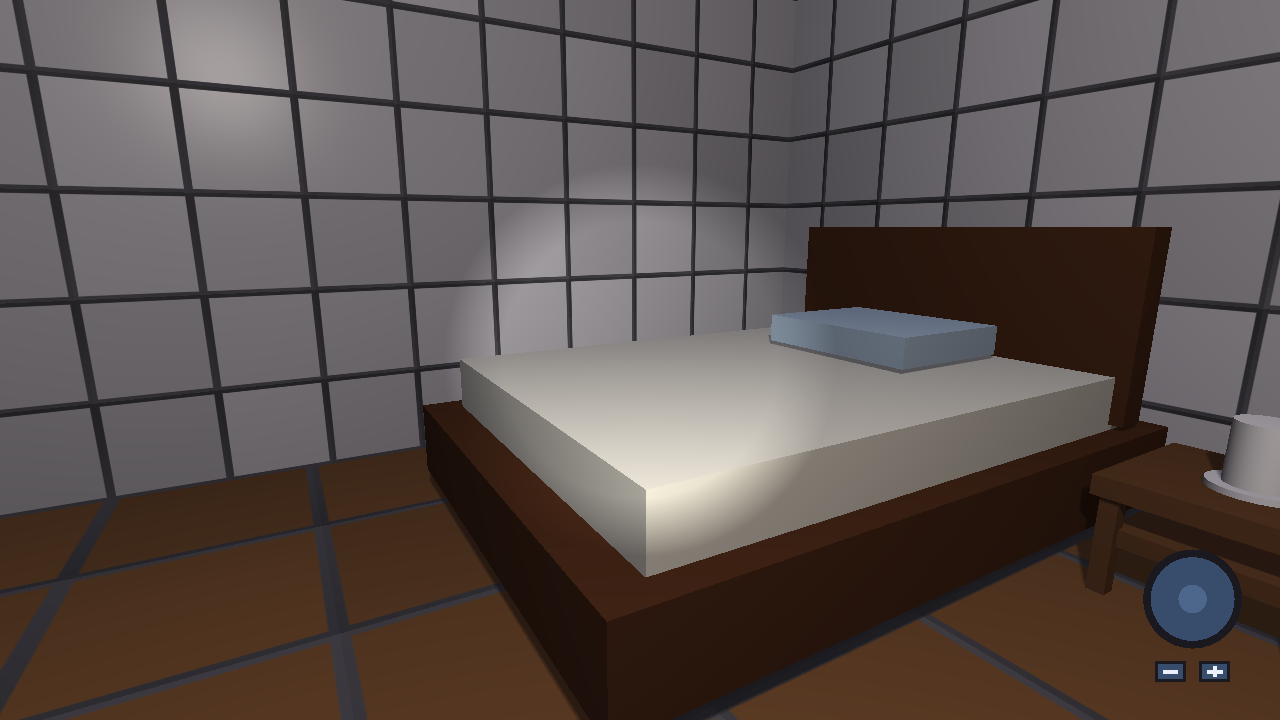
\includegraphics[width=0.85\textwidth]{shot_bed.png}
  \caption{Representative frame: bed and tea table area with tiled walls and soft shadow from table lamp.}
\end{figure}

\section{Benchmark methodology}
Performance was measured with a simple frame loop that rendered the scene repeatedly for a fixed number of frames while recording elapsed time and wall-clock memory. The default configuration used:
\begin{itemize}
  \item Window size: 1280 × 720
  \item Shadow map size: 2048 (main and lamp)
  \item V-Sync: enabled (swap interval = 1)
\end{itemize}
A typical run produced stable frame times around 16–18 ms on an integrated Intel GPU with shadow caching enabled, yielding approximately 55–60 FPS when vsync was not limiting; with vsync the observed frame rate was 60 FPS.

\section{Memory and GPU considerations}
Shadow map textures at 2048×2048 × depth24 consume GPU memory per map; two such maps are allocated by default. Reducing `SHADOW_MAP_SIZE` in `config/settings.py` reduces memory usage and improves performance at a cost to shadow quality.

\section{Lighting distribution analysis}
The ceiling/overhead light provides soft ambient illumination while the table lamp provides a localized warm highlight and soft shadowing. The glass window allows exterior panels to contribute light; translucency and Fresnel produce realistic reflections when viewed at glancing angles.

%-------------------------
% CHAPTER 8: CONCLUSION & FUTURE SCOPE
%-------------------------
\chapter{Conclusion \& Future Scope}

This lab project successfully demonstrates a compact but production-minded rendering architecture in Python and OpenGL. The key learning outcomes include shader-based procedural texturing, shadow mapping with PCF, layered rendering with transparent materials, and robust interactive controls suitable for 3D walkthroughs.

Future improvements:
\begin{itemize}
  \item Add normal maps and parallax occlusion mapping for richer tile detail.
  \item Implement clustered or tiled lighting for better scalability with many lights.
  \item Add HDR tone-mapping and bloom to increase realism.
  \item Port performance-critical code paths to C/C++ or use compute shaders for heavier effects.
\end{itemize}

%-------------------------
% OVERLEAF ASSET INTEGRATION
%-------------------------
\appendix
\chapter{Overleaf asset integration and diagrams}
Place the following images into `asset/overleaf/` so that the figures below compile cleanly in Overleaf.

\section{Room layout (top-down)}
\begin{figure}[H]
  \centering
  \includegraphics[width=\textwidth]{asset/overleaf/room_layout.png}
  \caption{Top-down schematic: bed, bookshelf/reading table, left-wall glass window, and tiled floor plan.}
\end{figure}

\section{Lighting distribution}
\begin{figure}[H]
  \centering
  \includegraphics[width=\textwidth]{asset/overleaf/lighting_distribution.png}
  \caption{Schematic showing attenuation circles for the ceiling point light and the warm table lamp and approximate shadow directions.}
\end{figure}

\section{Camera \& joystick pipeline}
\begin{figure}[H]
  \centering
  \includegraphics[width=\textwidth]{asset/overleaf/camera_joystick_pipeline.png}
  \caption{Data flow diagram: input events → InputManager → CameraControllerUI → Camera updates → view matrix.}
\end{figure}

\section{TikZ examples (optional)}
The following minimal TikZ diagram can be used as a starting point if a PNG is not available:
\begin{figure}[H]
  \centering
  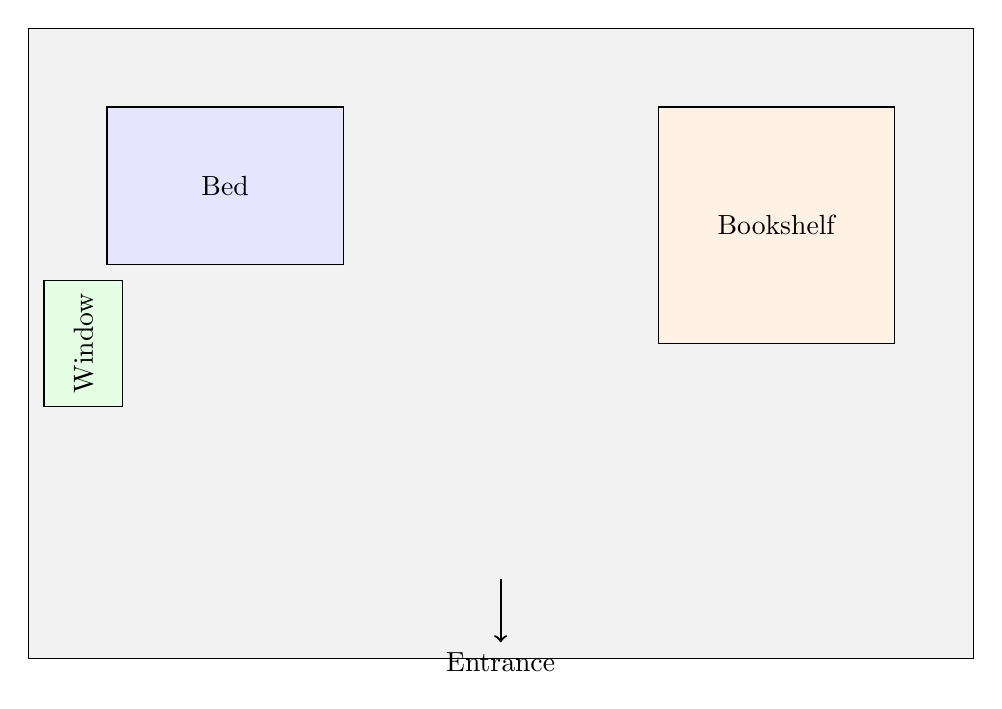
\begin{tikzpicture}[scale=1]
    \draw[fill=gray!10] (0,0) rectangle (12,8);
    \draw[fill=blue!10] (1,5) rectangle (4,7) node[midway]{Bed};
    \draw[fill=orange!10] (8,4) rectangle (11,7) node[midway]{Bookshelf};
    \draw[fill=green!10] (0.2,3.2) rectangle (1.2,4.8) node[midway,rotate=90]{Window};
    \draw[->,thick] (6,1) -- (6,0.2) node[below]{Entrance};
  \end{tikzpicture}
  \caption{Simple top-down sketch drawn with TikZ (for quick Overleaf prototyping).}
\end{figure}

\vfill
\end{document}

